We created a set of mockups to guide the implementation of the application's
user interface. These mockups served as visual representations of the intended
design and layout of the user interface, aiding in the visualisation and
communication of the desired interface elements and interactions. The mockups
acted as a blueprint for the development process, assisting the implementation
in achieving the envisioned user interface design.

\Cref{fig:mockup-tool-language-selection} primarily facilitates the selection
of the tool and programming language to be used, thereby addressing the
requirements FR01 and FR02. \Cref{fig:mockup-project-source-code-upload} is
dedicated to fulfilling FR05, which pertains to the capability of uploading the
project's source code. \Cref{fig:mockup-tool-parameter-tuning} addresses FR03,
which involves the ability to perform parameter tuning for each selected tool.
This figure showcases the user interface elements and options that enable users
to adjust and fine-tune parameters associated with the chosen tool.
\Cref{fig:mockup-decomposition-status} illustrates the provision of feedback
regarding the status of the decomposition process after the project upload.
This feedback mechanism keeps users informed about the progress and status of
the decomposition, allowing them to track the ongoing process.
\Cref{fig:mockup-decomposition-visualisation} focuses on the frontend's
capability to visualise the identified microservices and facilitate comparisons
between multiple identifications, addressing FR04 and FR06. This figure
demonstrates the user interface elements that enable users to visually explore
and analyse the identified microservices, supporting the comparative analysis
of different decompositions.

In \Cref{fig:mockup-decomposition-visualisation}, we propose representing each
microservice as a circular geometric shape, with the shape's size determined by
a metric derived from the underlying tool. This metric could be based on
factors such as the number of classes, the amount of code, or any other
relevant metric determined by the tool. Additionally, we aim to illustrate the
relationships between microservices within the visualisation by a line in which
microservice dependencies, call stacks, or data flow, among other factors,
define its stroke size.

\begin{figure*}[!htb]
  \centering
  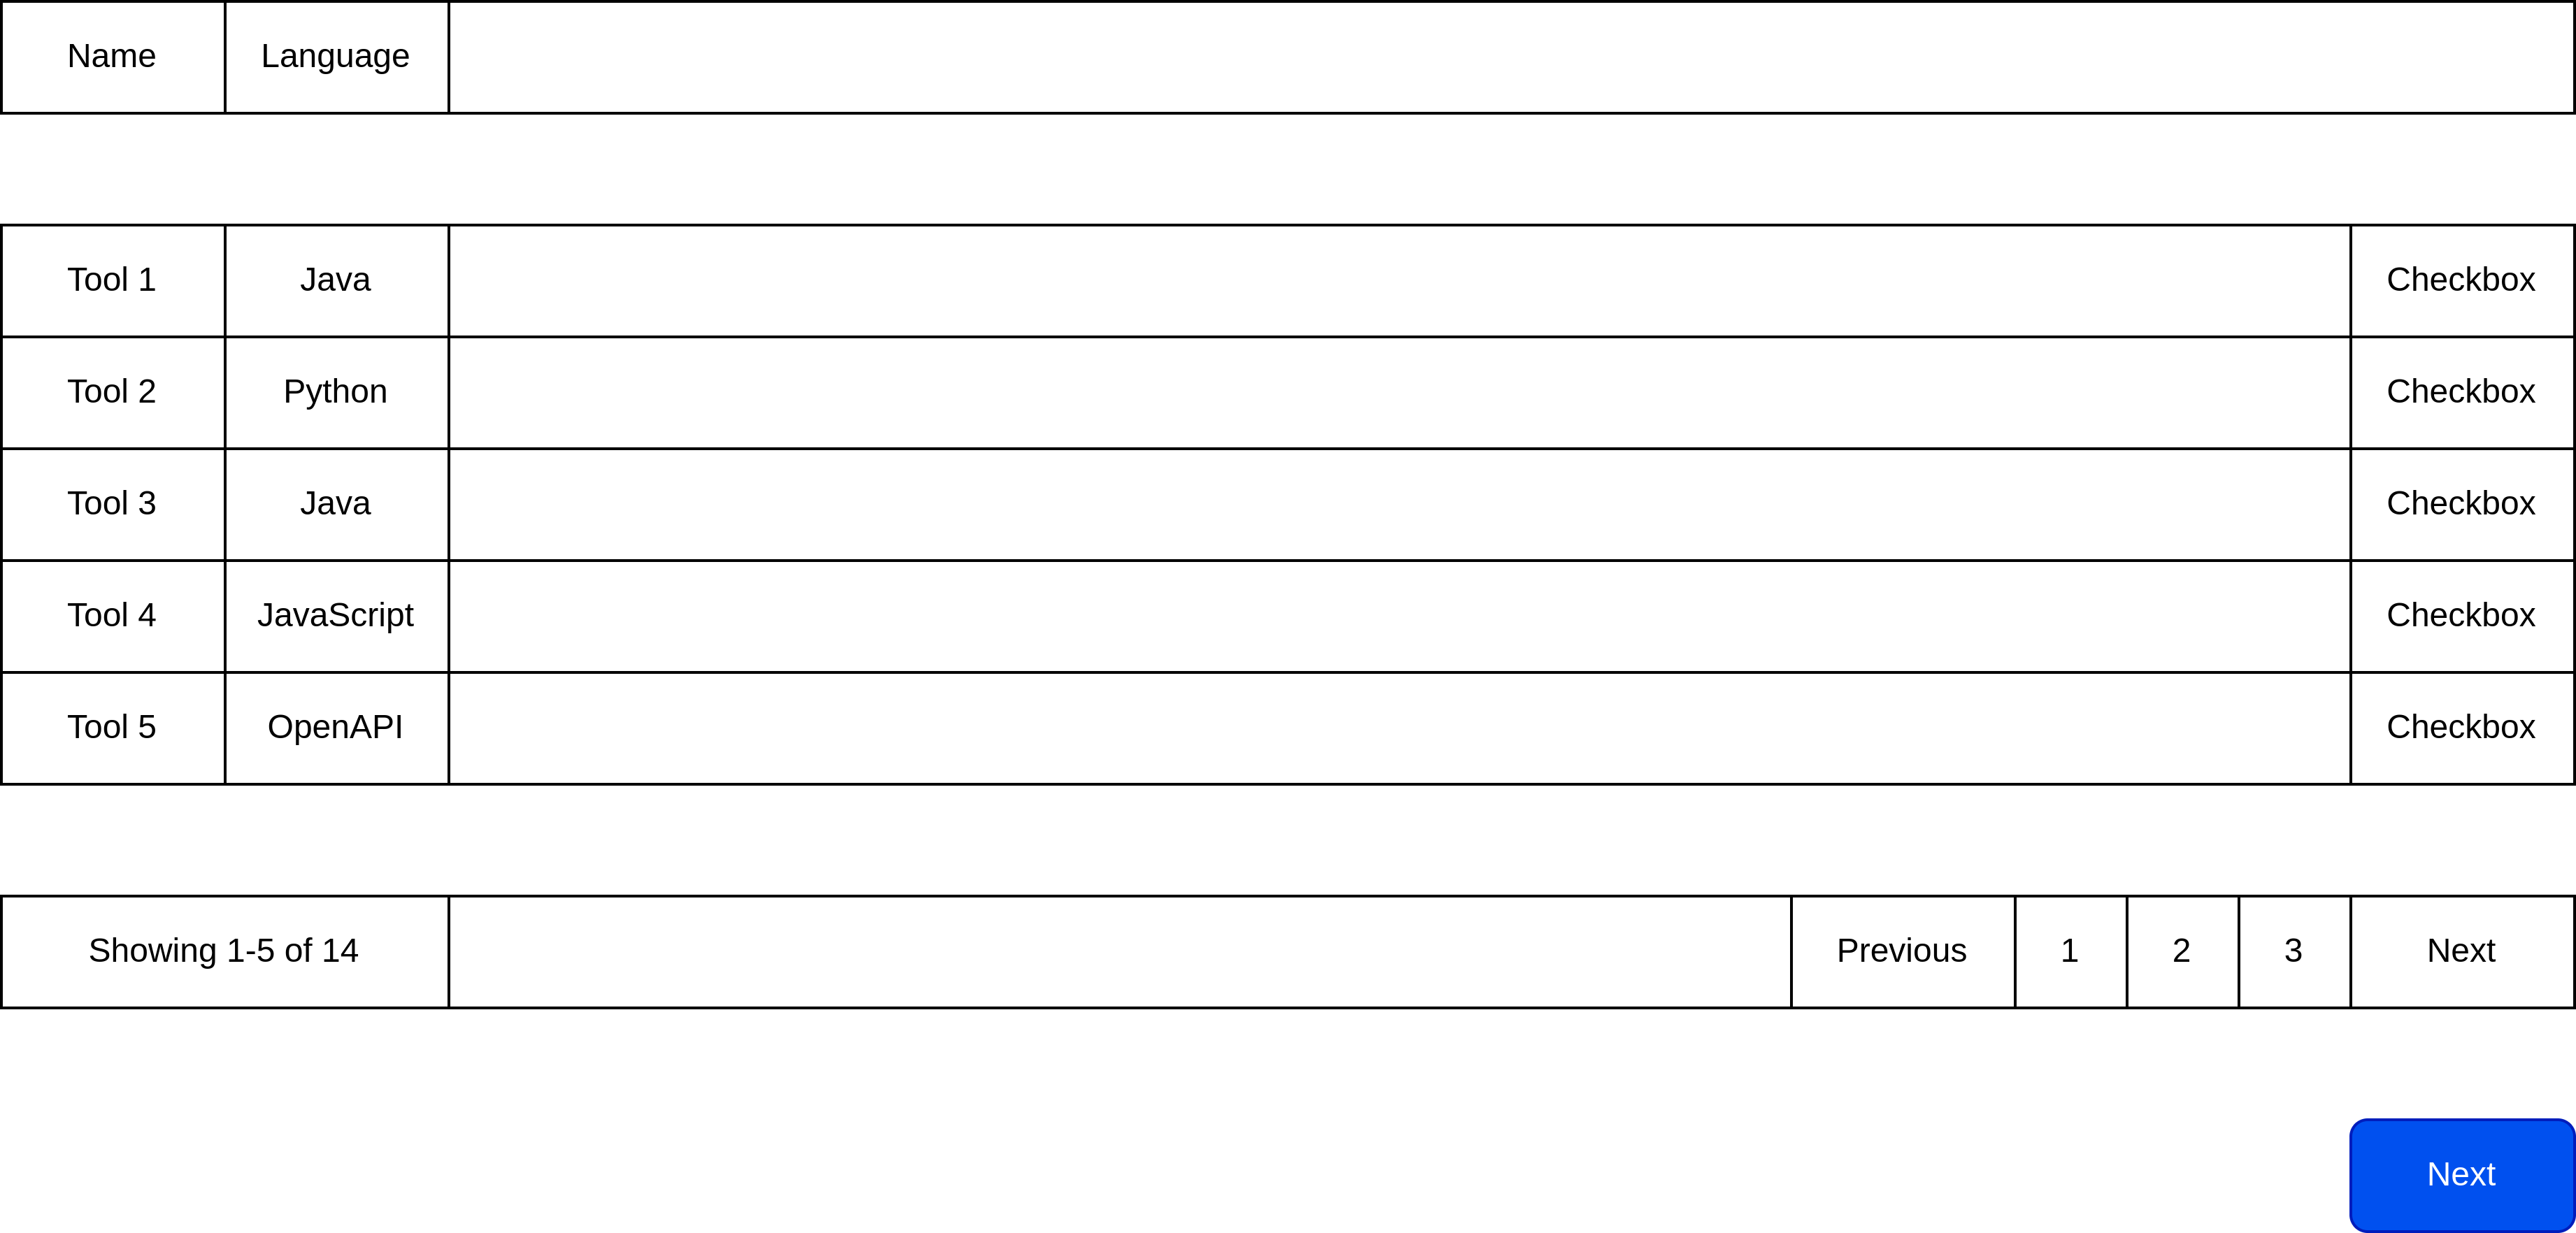
\includegraphics[width=\textwidth]{thesis-UI1.drawio}
  \caption{Tool/Language Selection}
  \label{fig:mockup-tool-language-selection}
\end{figure*}

\begin{figure*}[!htb]
  \centering
  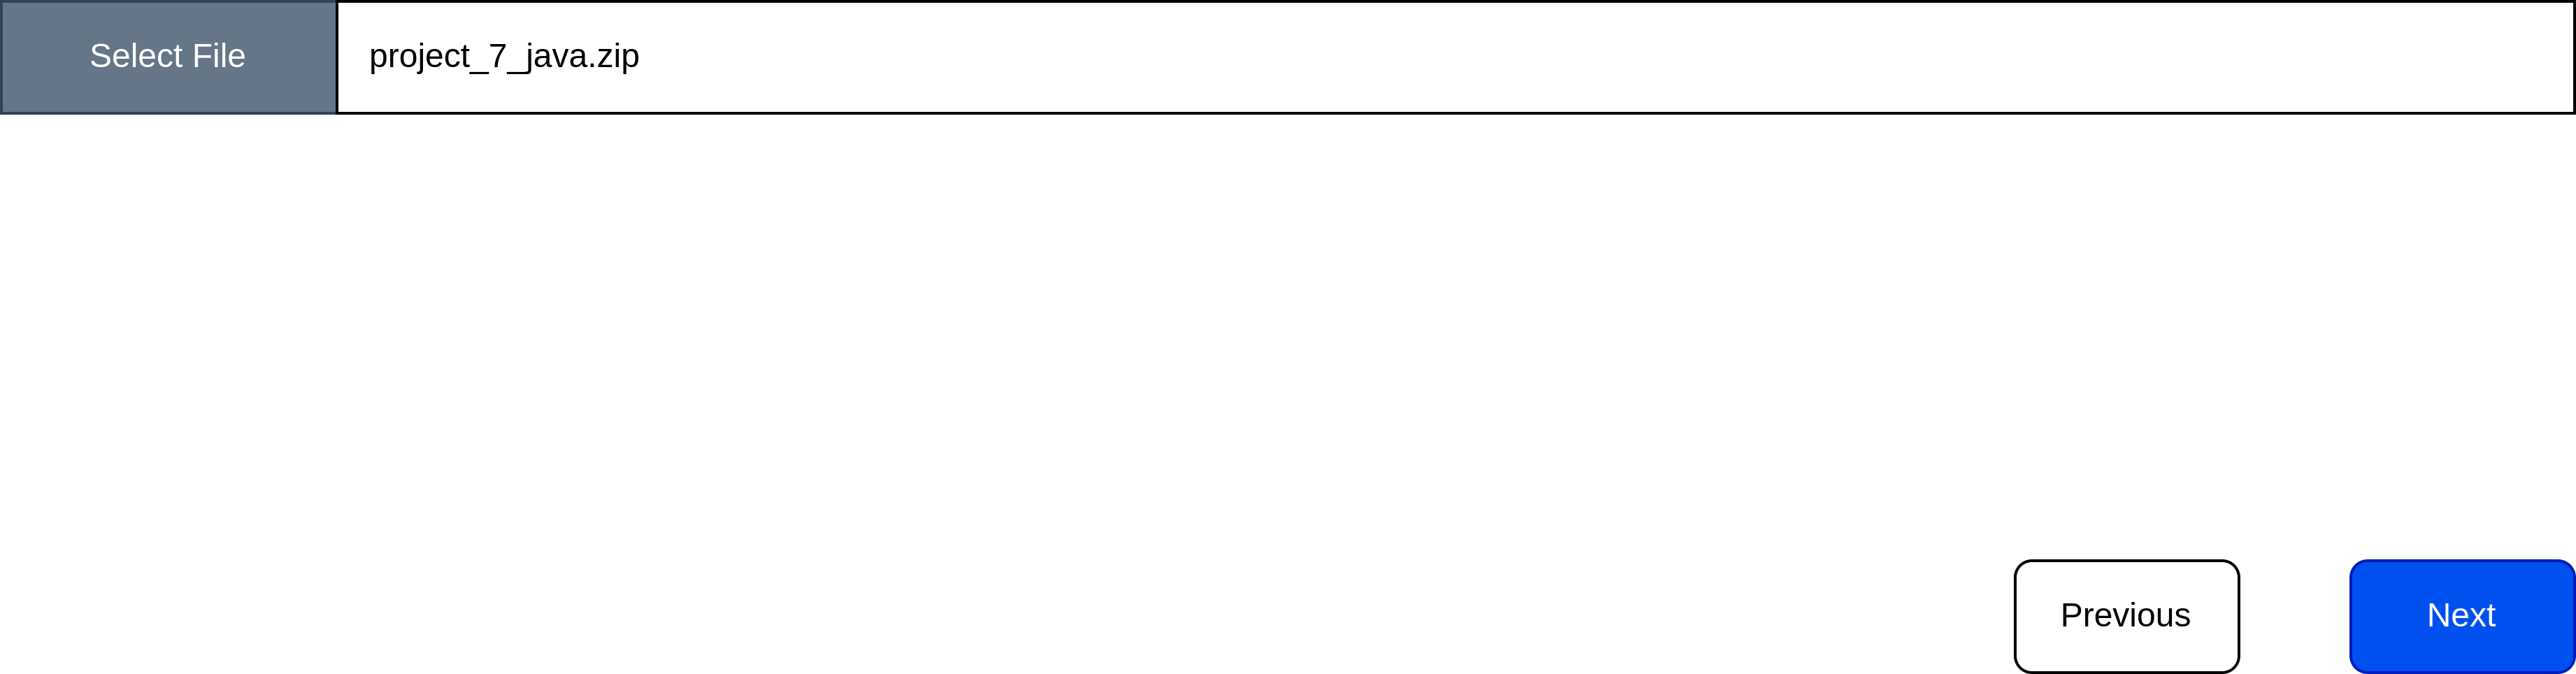
\includegraphics[width=\textwidth]{thesis-UI2.drawio}
  \caption{Project or Source Code upload}
  \label{fig:mockup-project-source-code-upload}
\end{figure*}

\begin{figure*}[!htb]
  \centering
  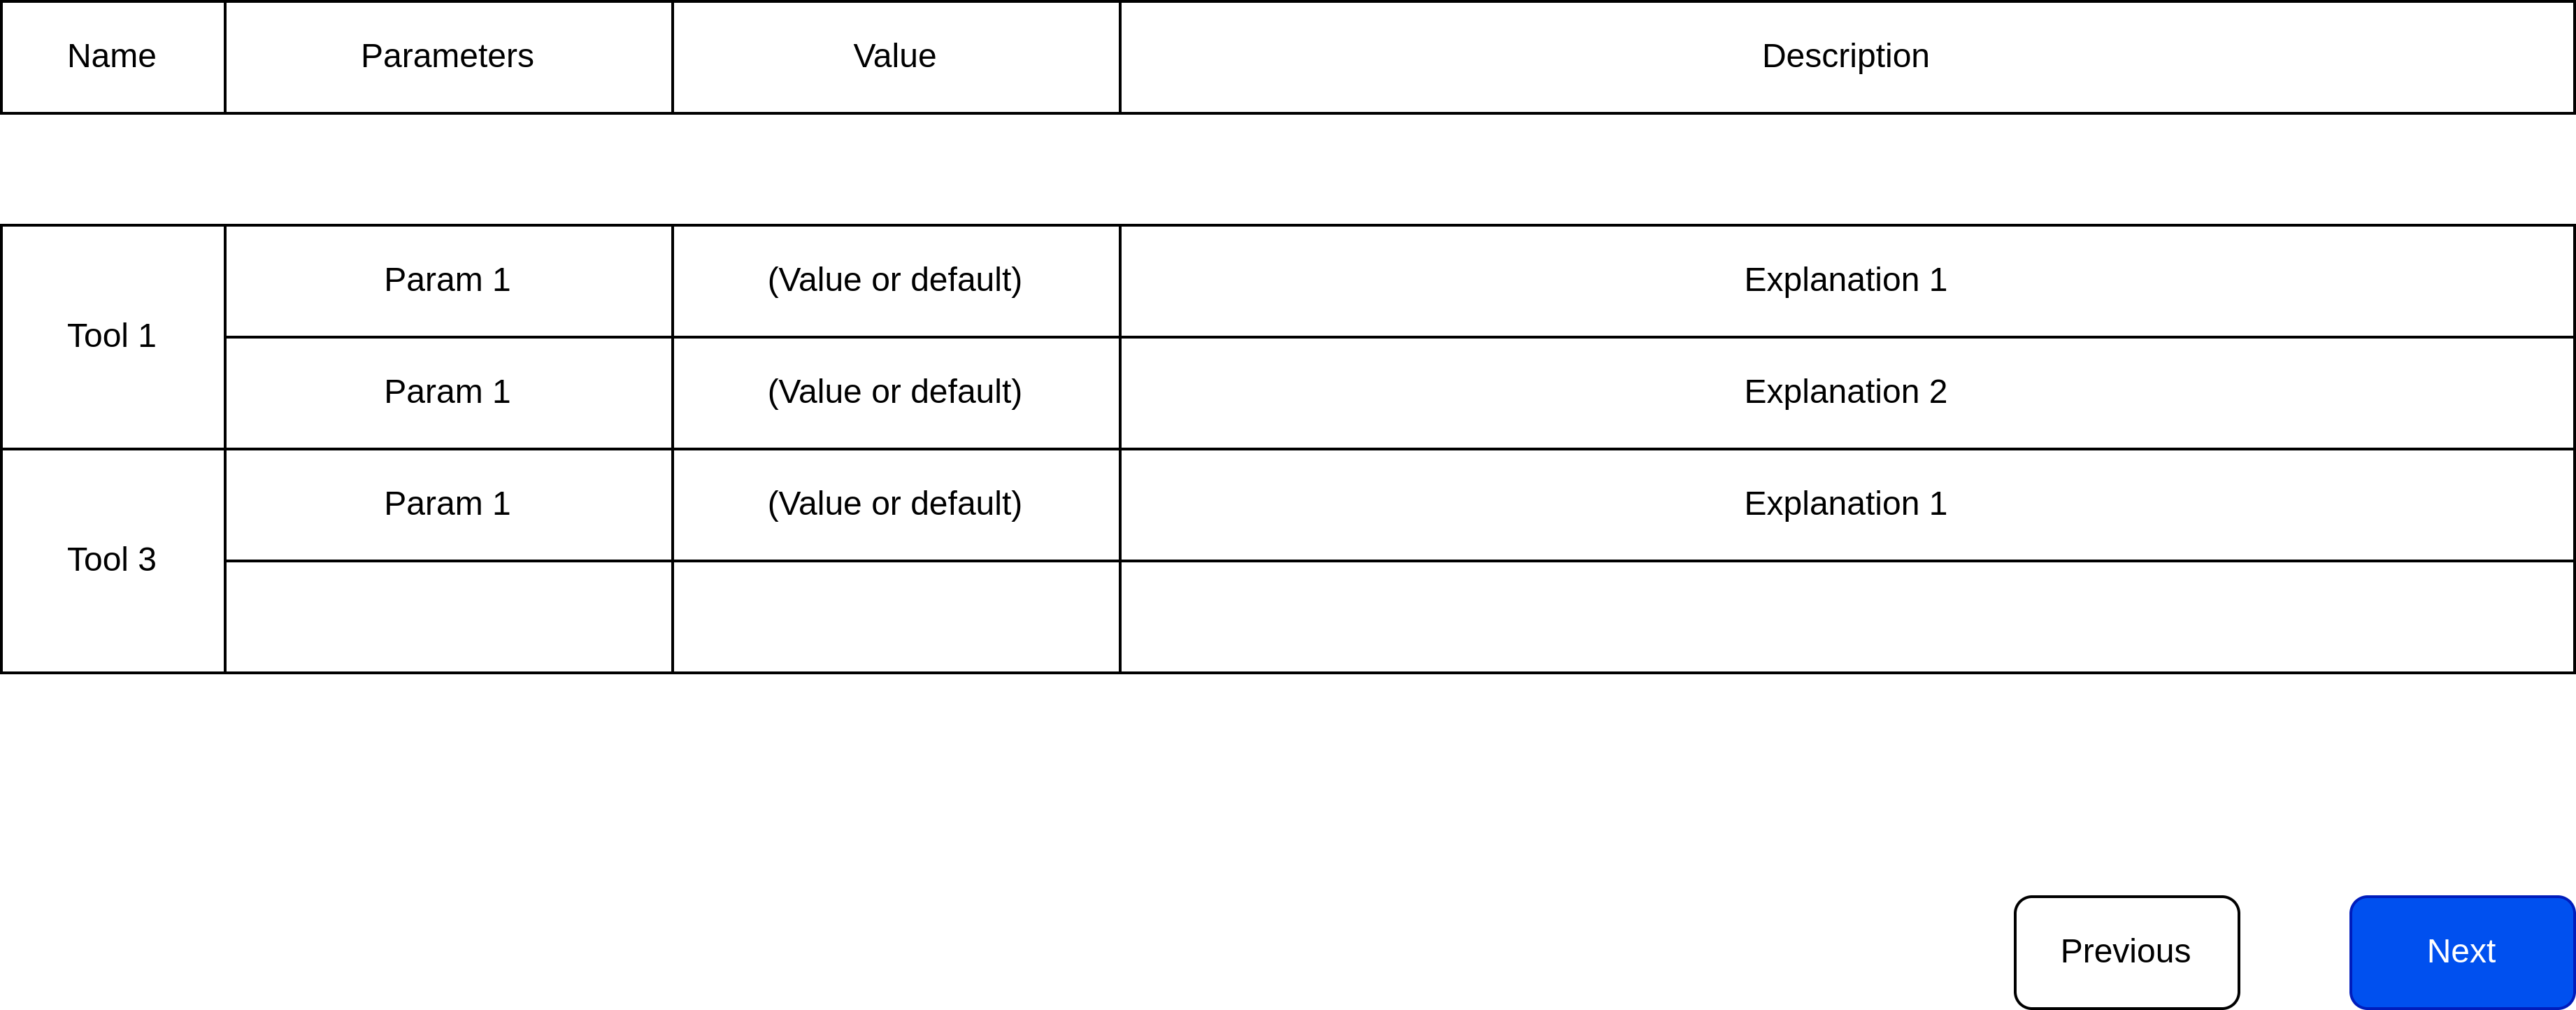
\includegraphics[width=\textwidth]{thesis-UI3.drawio}
  \caption{Per tool parameter tuning}
  \label{fig:mockup-tool-parameter-tuning}
\end{figure*}

\begin{figure*}[!htb]
  \centering
  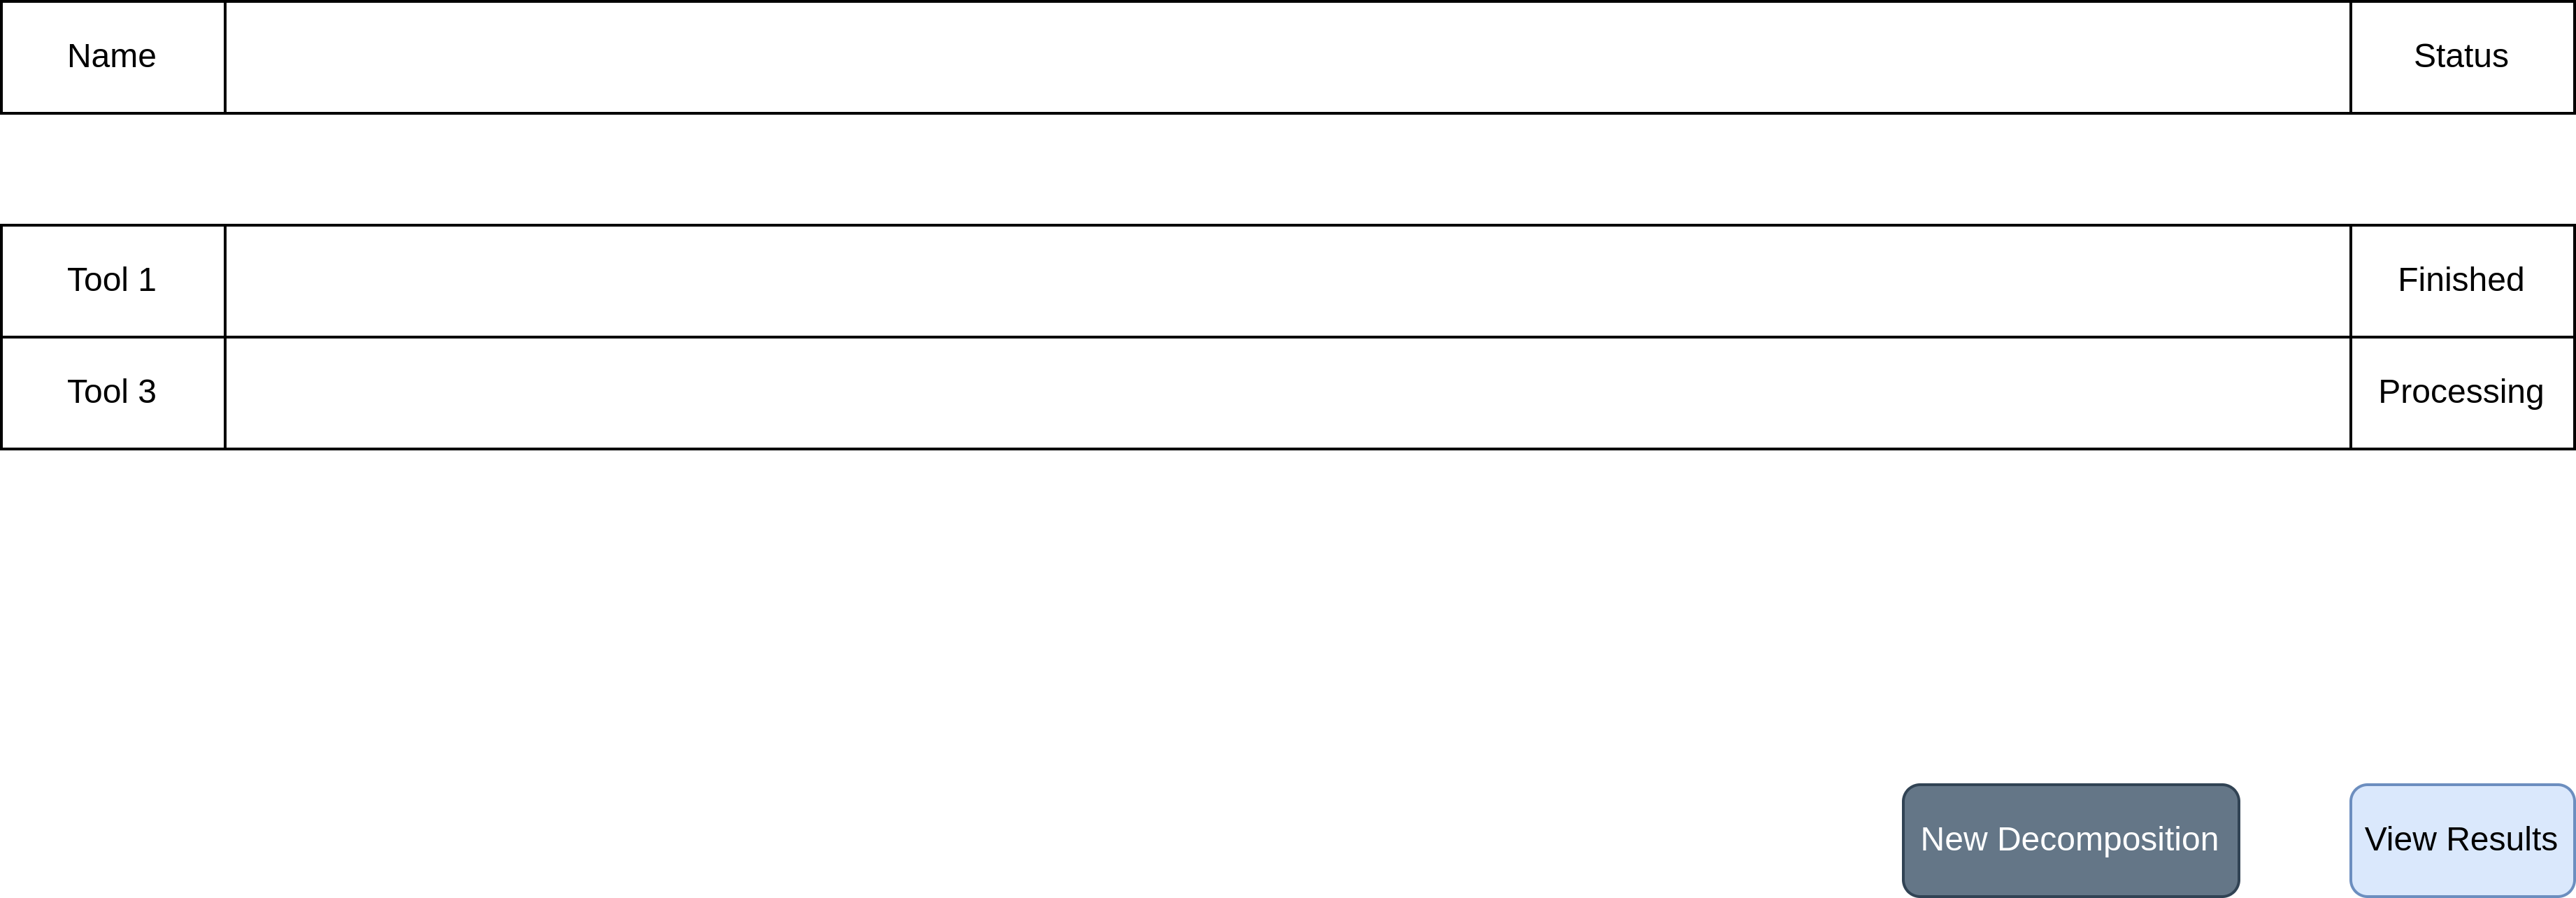
\includegraphics[width=\textwidth]{thesis-UI4.drawio}
  \caption{Decomposition Status}
  \label{fig:mockup-decomposition-status}
\end{figure*}

\begin{figure*}[!htb]
  \centering
  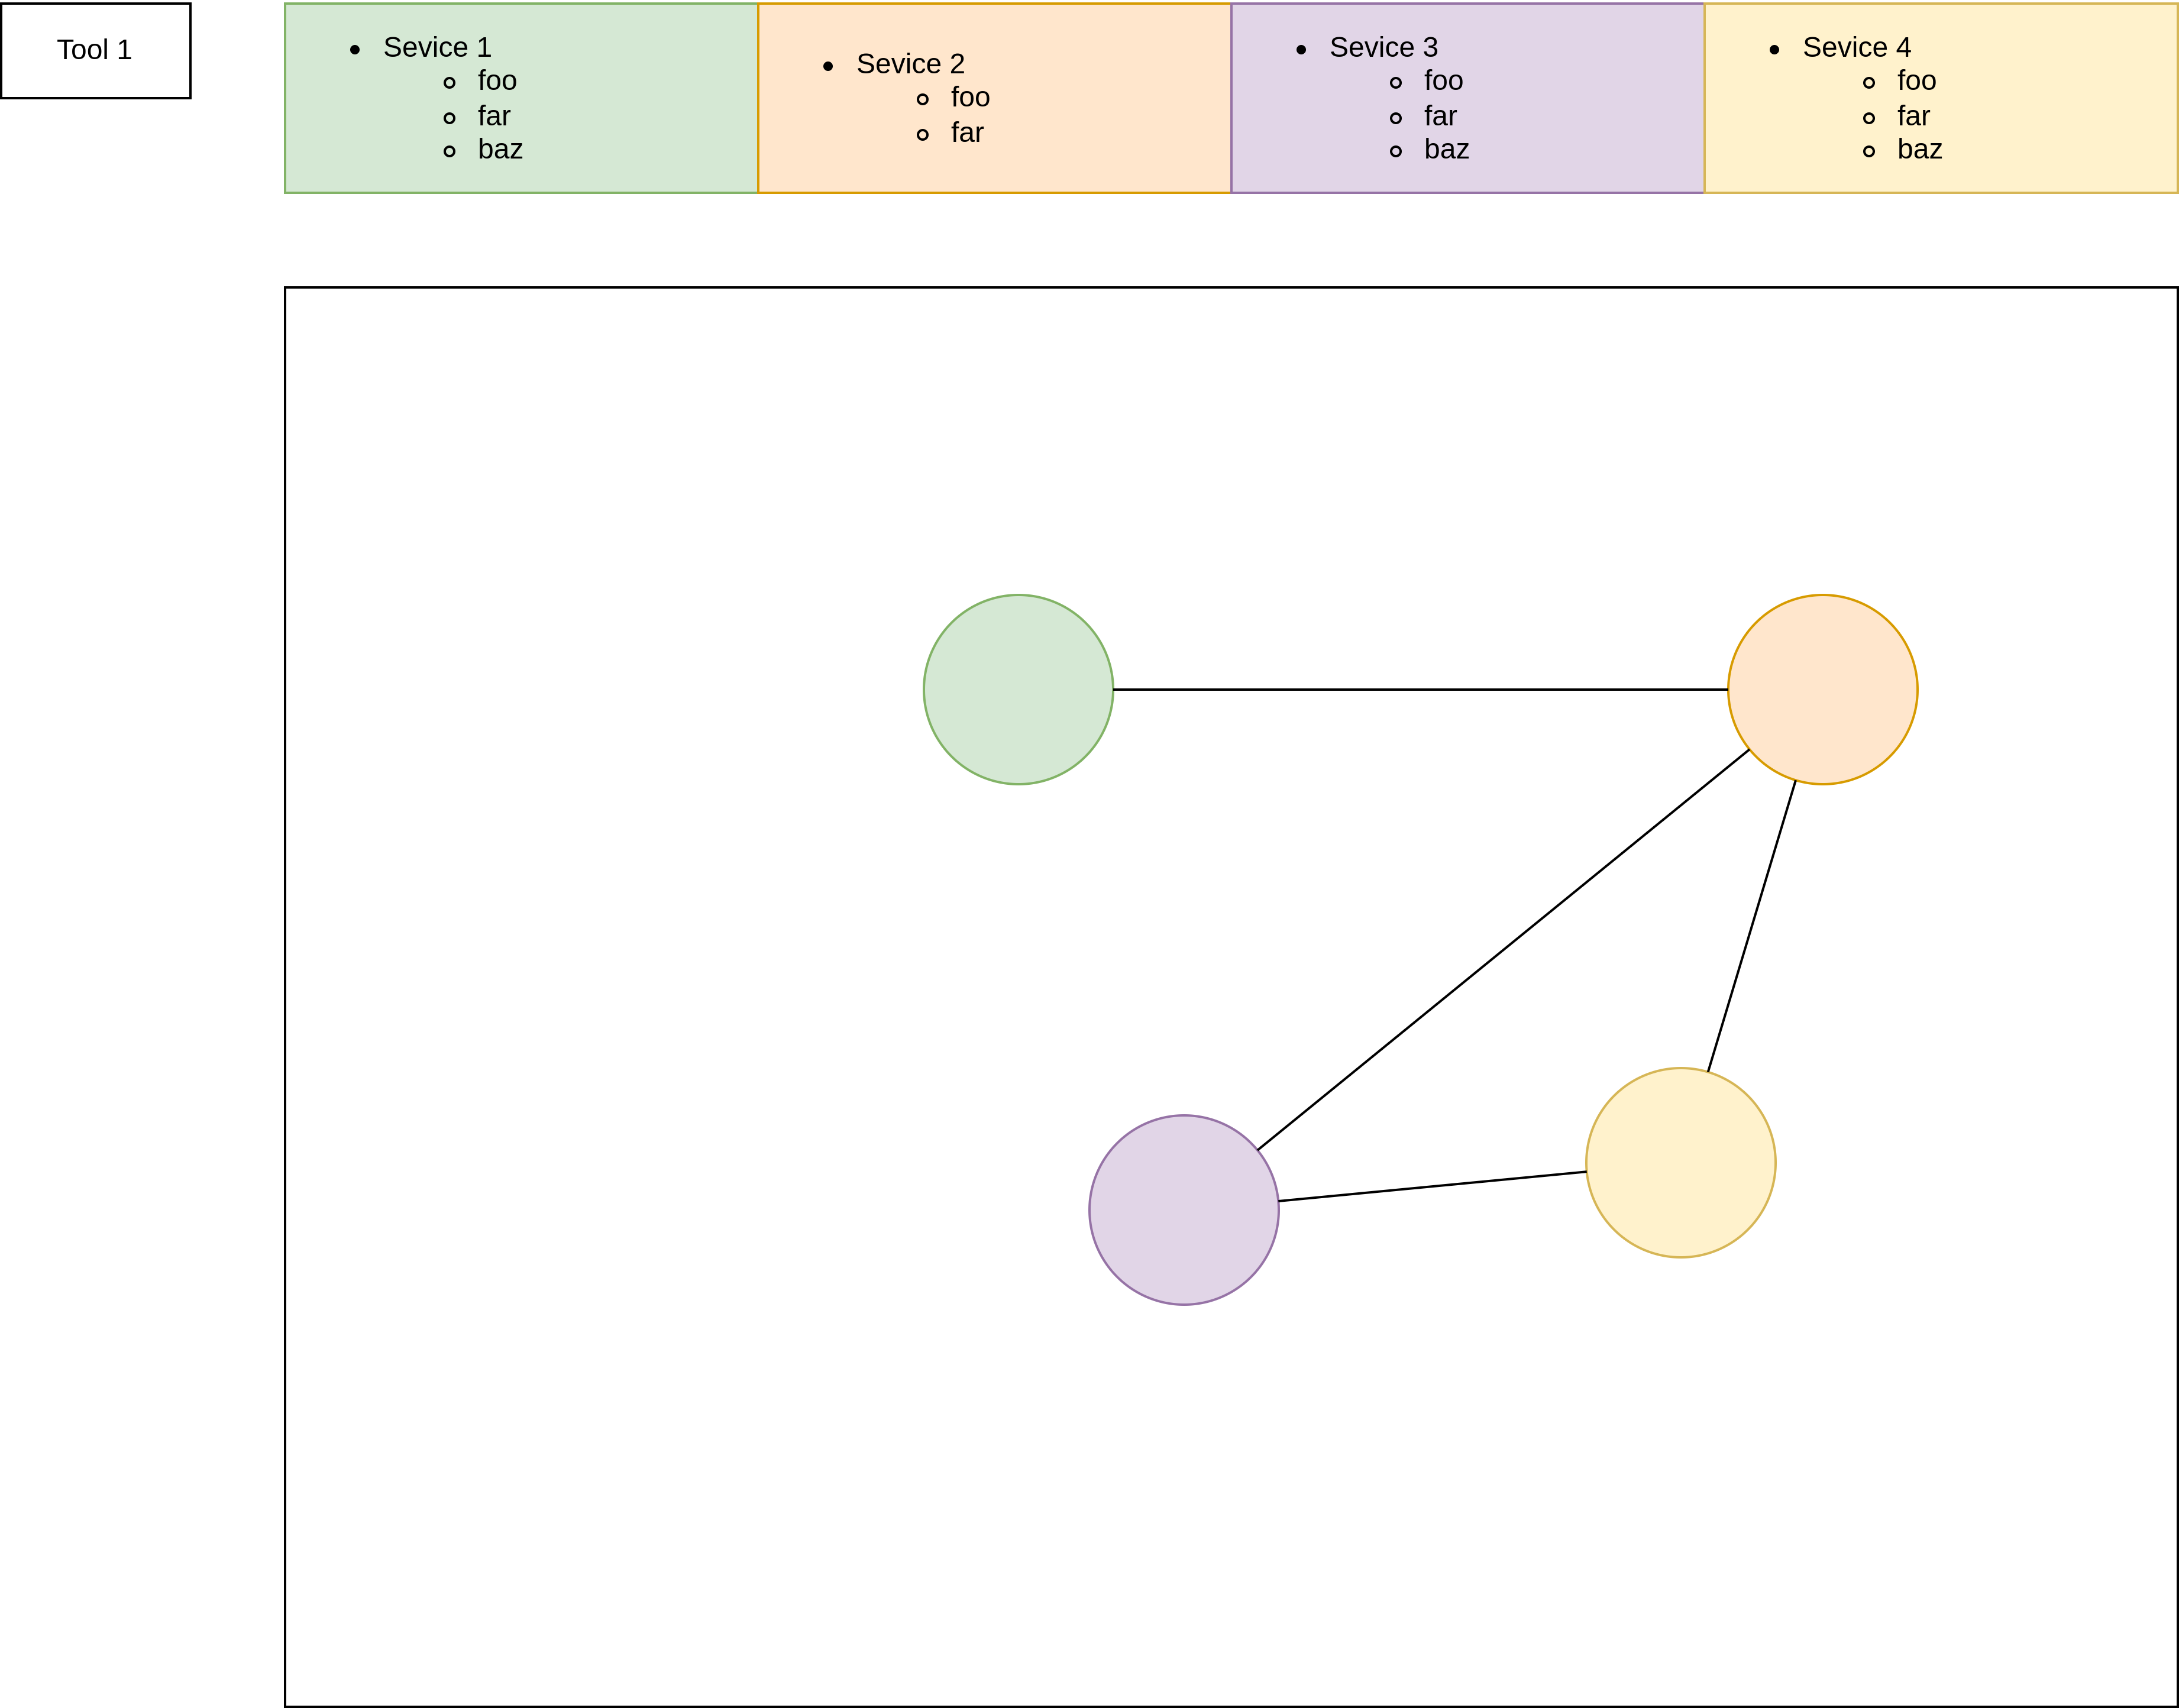
\includegraphics[width=\textwidth]{thesis-UI5.drawio}
  \caption{Decomposition Visualisation}
  \label{fig:mockup-decomposition-visualisation}
\end{figure*}
